\documentclass[10pt]{article}
\usepackage{CJKutf8}
\usepackage{hyperref}
\usepackage{graphicx}
\usepackage{float}

% can create colorful boxes, for warning p.ex.
\usepackage[most]{tcolorbox}

% making the text of the report sans serif
\renewcommand{\familydefault}{\sfdefault}

\title{Setting up and using Xilinx's KRIA KV260 board \\[1ex] \large \begin{CJK}{UTF8}{min}南山大学\end{CJK}}
\date{}
\author{Vincent Conus}

\begin{document}

\maketitle

\begin{figure}[H]
  \centering
  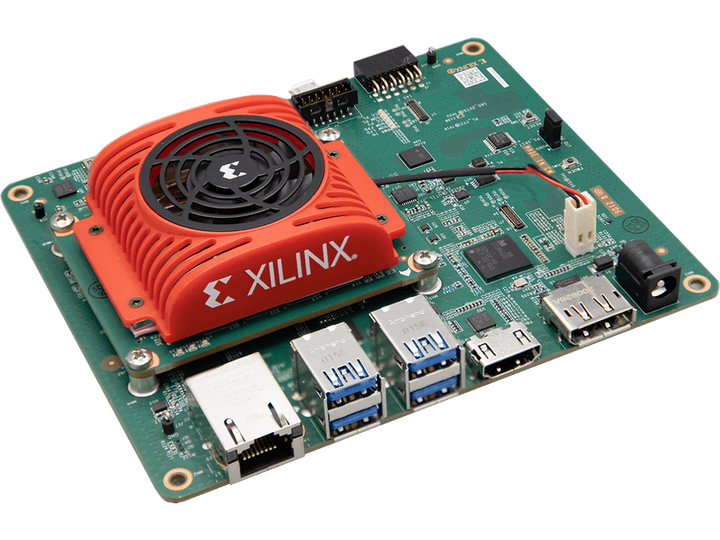
\includegraphics[width=0.8\textwidth]{./img/board}
\end{figure}

\pagebreak
\tableofcontents

\pagebreak
%-------------------------------------------------------------------------------
\section{Introduction and motivation}
\label{sec:intr-motiv}

\subsection{Documentation and guides}
\label{sec:documentation-guides}

\begin{itemize}
\item Board product information:\\ \url{https://www.xilinx.com/products/som/kria/kv260-vision-starter-kit.html}
\item SoC product information:\\ \url{https://www.xilinx.com/products/silicon-devices/soc/zynq-ultrascale-mpsoc.html}
\item Download page for the official Canonical Ubuntu releases for the board:\\ \url{https://ubuntu.com/download/amd-xilinx}
\item Xilinx official documentation:\\ \url{https://docs.xilinx.com/r/en-US/ug1089-kv260-starter-kit/Summary}
\item Atlassian documentation:\\ \url{https://xilinx-wiki.atlassian.net/wiki/spaces/A/pages/1641152513/Kria+K26+SOM}
\item Fixstar presentation (JP):\\  \url{https://speakerdeck.com/fixstars/fpga-seminar-12-fixstars-corporation-20220727}
\item Xilinx OpenAMP demo documentation:\\ \url{https://xilinx.github.io/kria-apps-docs/openamp/build/html/openamp\_landing.html}
\item Libmetal and OpenAMP official Xilinx documentation:\\ \url{https://docs.xilinx.com/r/en-US/ug1186-zynq-openamp-gsg/Introduction?tocId=GFruK4\_sY1eyu3jD9X1EuA}
\item Guide for KV260 board setup (JP):\\ \url{https://zenn.dev/ryuz88/articles/kv260\_setup\_memo\_ubuntu22}
\item Vitis IDE download page:\\ \url{https://www.xilinx.com/support/download/index.html/content/xilinx/en/downloadNav/vitis.html}
\end{itemize}


% -------------------------------------------------------------------------------
\section{Boot Image Update}
\label{sec:boot-image-update}
In order to be able to boot a newer version of Linux, the
boot image of the board must be updated.

The procedure is available in \href{https://docs.xilinx.com/r/en-US/ug1089-kv260-starter-kit/Firmware-Update}{the official documentation},
but I will present it step by step here.

%-------------------------------------------------------------------------------
\section{Ubuntu 22.04}
\label{sec:ubuntu-22.04}
\href{https://ubuntu.com/download/amd-xilinx}{An official image} is provided by Xilinx that allows the OS installation to be quick and
straightforward.

\begin{tcolorbox}[colback=red!5!white,colframe=red!75!black]
  WARNING: The next part involve the \verb|dd| command writing on disks!!! \\
  As always with the dd command, you have to be VERY careful on what arguments you give. Selecting the wrong disk will result on the destruction of your data !! \\
  \textbf{If you are unsure of what to do, seek assistance !}
\end{tcolorbox}


With the image available on you machine, one can simply run the \verb|dd| command as follow to write the image to a
previously formatted drive (here \verb|/dev/sda|). It is the possible to connect to the board using serial, as presented here:
\begin{tcolorbox}
\begin{verbatim}
sudo dd if=iot-limerick-kria-classic-desktop-2204-x07-\
20230302-63.img of=/dev/sda status=progress bs=8M && sync

sudo picocom /dev/ttyUSB1 -b 115200
\end{verbatim}
\end{tcolorbox}

Once logged in, it is typically easier and more convenient to connect the board using SSH.
When the board is connected to the network, it is possible to know it's IP address with
the \verb|ip| command; then it is possible to connect to the board with ssh, as follow (example):
\begin{tcolorbox}
\begin{verbatim}
kria# ip -a

host# ssh ubuntu@192.168.4.11
\end{verbatim}
\end{tcolorbox}

\subsection{Proxy and DNS}
\label{sec:proxy-dns}
Need to be set in order to be able to download stuff.

DNS in /etc/resolv.conf

proxy setup with export

% -------------------------------------------------------------------------------
\section{Starting remoteproc}
\label{sec:starting-remoteproc}
One of the advantage of this board, as cited previously, is the presence of
multiple types of core (APU, MCU, FPGA) on the same chip.

The part we are focusing in this guide is the usage of both the APU, running
a Linux distribution and ROS2; and the MCU, running FreeRTOS and micro-ROS.

The communication between both side is meant to be done using shared memory, but
some extra setup is required.
This section will present how to setup and use as an example the \verb|remoteproc|
and RPMsg system.

\subsection{References}
\label{sec:referances}
This exact use-case is not exactly presented in the official documentation, but some
guides were found to eventually put together this procedure.

\begin{itemize}
\item \href{https://speakerdeck.com/fixstars/fpga-seminar-12-fixstars-corporation-20220727}{A slideshow (JP) from Fixstar employees} presents how
  to use the device tree to enable the communication between the cores.
\item \href{https://zenn.dev/ryuz88/articles/kv260_setup_memo_ubuntu22}{This blog article (JP)} shows all the major steps on how to enable the \verb|remoteproc|.
\end{itemize}


\subsection{DTO patching}
\label{sec:dto-patching}

\begin{tcolorbox}
\begin{verbatim}
sudo dtc /sys/firmware/fdt 2> /dev/null > system.dts
\end{verbatim}
\end{tcolorbox}

\begin{tcolorbox}
\begin{verbatim}
patch
\end{verbatim}
\end{tcolorbox}

Now the DTS file has been modified, one can regenerate the binary and place it on the \verb|/boot| partition
and reboot the board.
\begin{tcolorbox}
\begin{verbatim}
dtc -I dts -O dtb system.dts -o user-override.dtb
sudo cp user-override.dtb /boot/firmware/
sudo reboot now
\end{verbatim}
\end{tcolorbox}

After rebooting, you can check the content of the \verb|remoteproc| system directory,
and a \verb|remoteproc0| device should be visible, as follow.
\begin{tcolorbox}
\begin{verbatim}
ls /sys/class/remoteproc/
#  remoteproc0
\end{verbatim}
\end{tcolorbox}

If it is the case, it means that the patch was successful and RPMsg is
ready to test with some example.

\subsection{Ping-pong example}
\label{sec:ping-pong-example}





% -------------------------------------------------------------------------------
\section{ROS2}
\label{sec:ros2}
As an Ubuntu distribution is installed on the board, the installation of ROS2 can be done
in a standard way, using the repository.

An \href{https://docs.ros.org/en/humble/Installation/Ubuntu-Install-Debians.html}{official documentation}
is provided with ROS2 themselves with a step-by-step guide on how to install
ROS2 on a Ubuntu system\footnote{The curl command from the guide does not work through the school proxy,
  but the command wget used instead does work. The key is then moved to the correct spot with mv}.
We will follow this guide here.

Firstly, we need to update the locals,  enable the universe Ubuntu repository, get the key and add the repository for ROS2. This can be done as follow:

\begin{tcolorbox}
\begin{verbatim}
locale  # check for UTF-8
sudo apt update && sudo apt install -y locales
sudo locale-gen en_US en_US.UTF-8
sudo update-locale LC_ALL=en_US.UTF-8 LANG=en_US.UTF-8
export LANG=en_US.UTF-8
locale  # verify settings
sudo apt install -y software-properties-common
sudo add-apt-repository universe
sudo apt update && sudo apt install -y curl wget
wget https://raw.githubusercontent.com/ros/rosdistro/\
master/ros.key
sudo mv ros.key /usr/share/keyrings/ros-archive-keyring.gpg
\end{verbatim}
\end{tcolorbox}


This is a one-liner to add the ROS2 repository:

\begin{tcolorbox}
\begin{verbatim}
echo "deb [arch=$(dpkg --print-architecture) \
signed-by=/usr/share/keyrings/ros-archive-keyring.gpg] \
http://packages.ros.org/ros2/ubuntu $(. \
/etc/os-release && echo $UBUNTU_CODENAME) main" | \
sudo tee /etc/apt/sources.list.d/ros2.list > /dev/null
\end{verbatim}
\end{tcolorbox}

It is then possible to install ROS2\footnote{This command installs a complete ``desktop'' version of ROS2. If space is a constraint, different, less complete packages can be install. Please refer to the official documentation about it.} as follow:

\begin{tcolorbox}
\begin{verbatim}
sudo apt update
sudo apt upgrade -y
sudo apt install -y ros-humble-desktop \
ros-humble-ros-base \
python3-argcomplete \
ros-dev-tools
\end{verbatim}
\end{tcolorbox}

Once installed, it is possible to test the system with a provided example. You need to open two terminals and log wish SSH onto the board, then running respectively:

\begin{tcolorbox}
\begin{verbatim}
source /opt/ros/humble/setup.bash
ros2 run demo_nodes_cpp talker
\end{verbatim}
\end{tcolorbox}



\begin{tcolorbox}
\begin{verbatim}
source /opt/ros/humble/setup.bash
ros2 run demo_nodes_py listener
\end{verbatim}
\end{tcolorbox}


You should be able to see the first terminal sending "Hello world" messages, and the second one receiving then.


% -------------------------------------------------------------------------------
\section{Vitis IDE}
\label{sec:vitis-ide}
This is the recommended IDE used to build software for the Xilinx boards.
It also include the tools to interact with the FPGA part, making the whole
software very large (>200GB).

The installer can be found on \href{Xilinx download page}{https://www.xilinx.com/support/download/index.html/content/xilinx/en/downloadNav/vitis.html}. You will need to get
a file named something like ``Xilinx\_Unified\_2022.2\_1014\_8888\_Lin64.bin''.

Vitis IDE installer is compatible with versions of Ubuntu, among other distributions,
but not officially yet for the 22.04 version.
Furthermore, the current install was tested on Pop OS, a distribution derived from Ubuntu.

This guide will present a guide that supposedly works for all distributions based on the newest
LTS from Ubuntu.

\begin{tcolorbox}
\begin{verbatim}
sudo apt-get update
sudo apt-get install libncurses-dev \
ncurses-term \
ncurses-base \
ncurses-bin \
libncurses5 \
libtinfo5 \
libncurses5-dev \
libncursesw5-dev
\end{verbatim}
\end{tcolorbox}

\begin{tcolorbox}
\begin{verbatim}
./Xilinx_Unified_2022.2_1014_8888_Lin64.bin
\end{verbatim}
\end{tcolorbox}


% -------------------------------------------------------------------------------
\section{Building an example firmware}
\label{sec:bulding-an-example}
\href{Xilinx documentation about building a demo firmware}{https://xilinx-wiki.atlassian.net/wiki/spaces/A/pages/1837006921/OpenAMP+Base+Hardware+Configurations\#Build-RPU-firmware}

\subsection{Generating the platform configuration file}
\label{sec:gener-platf-conf}

\url{https://xilinx.github.io/kria-apps-docs/kv260/2022.1/build/html/docs/build_vitis_platform.html?highlight=xsa}

\url{https://github.com/Xilinx/kria-vitis-platforms}

\begin{tcolorbox}
\begin{verbatim}
git clone --recursive https://github.com/Xilinx/kria-vitis-platforms.git
cd kria-vitis-platforms/k26/platforms
export XILINX_VIVADO=/home/sunoc/Xilinx/Vivado/2022.2/
export XILINX_VITIS=/home/sunoc/Xilinx/Vitis/2022.2/
make platform PLATFORM=k26_base_starter_kit
\end{verbatim}
\end{tcolorbox}

Cmake, tcl and idn will become needed in order to build the firmware.
As discussed in a thread on \href{Xilinx community forum}{https://support.xilinx.com/s/question/0D52E00006jrzsYSAQ/platform-project-cannot-be-created-on-vitis?language=en\_US}, \verb|libidn11| is specifically required, but
creating a symbolic link from the current, 12 version works.
\begin{tcolorbox}
\begin{verbatim}
sudo apt-get update
sudo apt-get install cmake tcl libidn11-dev libidn-dev libidn12 idn
sudo ln -s /usr/lib/x86_64-linux-gnu/libidn.so.12 /usr/lib/x86_64-linux-gnu/libidn.so.11
\end{verbatim}
\end{tcolorbox}

% -------------------------------------------------------------------------------
\section{RPMsg}
\label{sec:rpmsg}

Get a readable copy of the device tree overlay:
\begin{tcolorbox}
\begin{verbatim}
sudo dtc /sys/firmware/fdt 2> /dev/null > system.dts
\end{verbatim}
\end{tcolorbox}

Patch it:

Re-generate the device tree binary and put in on the boot partition:

Reboot the board:

Check if the ~remoteproc~ was successfully loaded:

% -------------------------------------------------------------------------------
\section{Loading a new firmware from Linux}
\label{sec:loading-new-firmware}


\begin{tcolorbox}
\begin{verbatim}
sudo -s
echo image_echo_test  > /sys/class/remoteproc/remoteproc0/firmware
echo start > /sys/class/remoteproc/remoteproc0/state
echo_test
echo stop > /sys/class/remoteproc/remoteproc0/state
\end{verbatim}
\end{tcolorbox}




\end{document}